\documentclass{beamer}
\usepackage{amsmath,amssymb,amsthm,mathtools}
\usepackage{xcolor}
\usepackage{tikz}

\DeclareRobustCommand{\ReLU}{\mathrel{\text{%
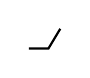
\begin{tikzpicture}[baseline=(current bounding box.south)]
    \draw[thick] (0,0) -- (0.25,0) -- (0.4,0.25);
\end{tikzpicture}}}\!\!}



\usetikzlibrary{positioning,shadows}
\usetheme{Madrid}

% Définition des couleurs
\definecolor{kernelcolor}{RGB}{220,20,60}
\definecolor{sobolevcolor}{RGB}{30,144,255}
\definecolor{weightcolor}{RGB}{101,67,33}
\definecolor{k3color}{RGB}{148,0,211}

% Commandes personnalisées
\newcommand{\E}{\mathbb{E}}

\newcommand{\K}{\textcolor{kernelcolor}{K}}
\newcommand{\NTK}{\textcolor{kernelcolor}{\mathbf{K}}}
\newcommand{\Ps}{\textcolor{sobolevcolor}{P_s}}

\title{Neural Tangent Kernel: Deeper or Wider?}
\author{Janis AIAD}
\institute{École Polytechnique \& University of Maryland}
\date{}

\begin{document}


\begin{frame}
\frametitle{Plan de la Présentation}

\begin{enumerate}
    \item \textbf{Introduction}
    \item \textbf{Sobolev training}
    \begin{itemize}
        \item Énoncé du problème
        \item Résultats et intuition pour les praticiens
    \end{itemize}
    
    \vspace{0.3cm}
    
    \item \textbf{Préconditionnement \& NTK/NTH}
    \begin{itemize}
        \item Pourquoi les MMNNs \& Transformers
        \item Éléments comparatifs
        \item Spécificités \& résultats        
    \end{itemize}
    
    \vspace{0.3cm}
    
    \item \textbf{Largeur Finie \& RMT}
    \begin{itemize}
        \item NTH pour réseau fini
        \item Intuition et découvertes
        \item Vers où et avec qui aller ensuite ?
    \end{itemize}
\end{enumerate}

\end{frame}



% Slide 1: Titre
\begin{frame}
\titlepage
\end{frame}

% Slide 2: Point de départ - Scaling Laws
\begin{frame}{Point de Départ}
\begin{center}
\textbf{Scaling Laws d'OpenAI}

\vspace{1cm}

Au-delà des 100k GPU:\\
Comment choisir en pratique\\
la taille optimale d'un réseau?

\vspace{0.5cm}

\textbf{SciML} : théorie $\leftrightarrow$ pratique
\end{center}
\end{frame}

% Slide 3: Méthodologie - 3 papiers
\begin{frame}{Méthodologie}
\begin{center}
\textbf{3 références initiales}

\vspace{0.5cm}

\textbf{1)} Sobolev training\\
\textbf{2)} MMNN \& Transformers\\
\textbf{3)} Finite-width corrections

\vspace{1cm}

\textbf{Conjecture:} NTK décrit le loss landscape\\
Analyses locales $\rightarrow$ globales
\end{center}
\end{frame}


% Slide 5: Espace de Sobolev
\begin{frame}{Norme de Sobolev}
\textbf{Norme gradient:}
\begin{equation}
\|f\|_{L^s}^2 = \sum_{p=0}^s \int_{\Omega} |D^p f(x)|^2 dx
\end{equation}

\textbf{Norme Fourier:}
\begin{equation}
\|f\|_{L^s}^2 = \int_{\mathbb{R}^d} (1 + |\xi|^2)^s |\hat{f}(\xi)|^2 d\xi
\end{equation}
\end{frame}

% Slide 6: Fonctions de perte
\begin{frame}{Loss Functions}

\textbf{Sobolev augmenté (PINNs):}
$$\mathcal{L}_{\text{deriv}}(f) = \sum_{i=1}^{n} \left(|f(x_i) - y_i|^2 + \sum_{p=1}^s |D^p f(x_i) - D^p y_i|^2\right)$$


\textbf{Regression standard:}
$$\mathcal{L}_{\text{MSE}}(f) = \sum_{i=1}^{n} |f(x_i) - y_i|^2$$
Analyse en fourier pertinente si assez de données sur sphere ($l_{max} \sim N^d$)
\end{frame}



% Slide 4: Résultats de Terjek
\begin{frame}{Résultats Théoriques}
    \textbf{Si beaucoup de points:} contraindre l'espace modèle
    
    $$\mu_\ell = \frac{\ell^s}{n}$$
    
    \vspace{0.5cm}
    
    Information de \textit{smoothness} dans les données\\
    $\Rightarrow$ éviter directions inutiles de l'espace paramètres
    
    \vspace{0.5cm}
    
    \textbf{Contribution:} bornes explicites avec Haizhao Yang, \\
    Futur borne pour toute distribution sur $\mathbb{S}^{d-1}$
\end{frame}



% Slide 7: Préconditionnement - MMNN
\begin{frame}{MMNN : Multi-Component Networks}

%figure landscape mmnn
\begin{figure}
\centering
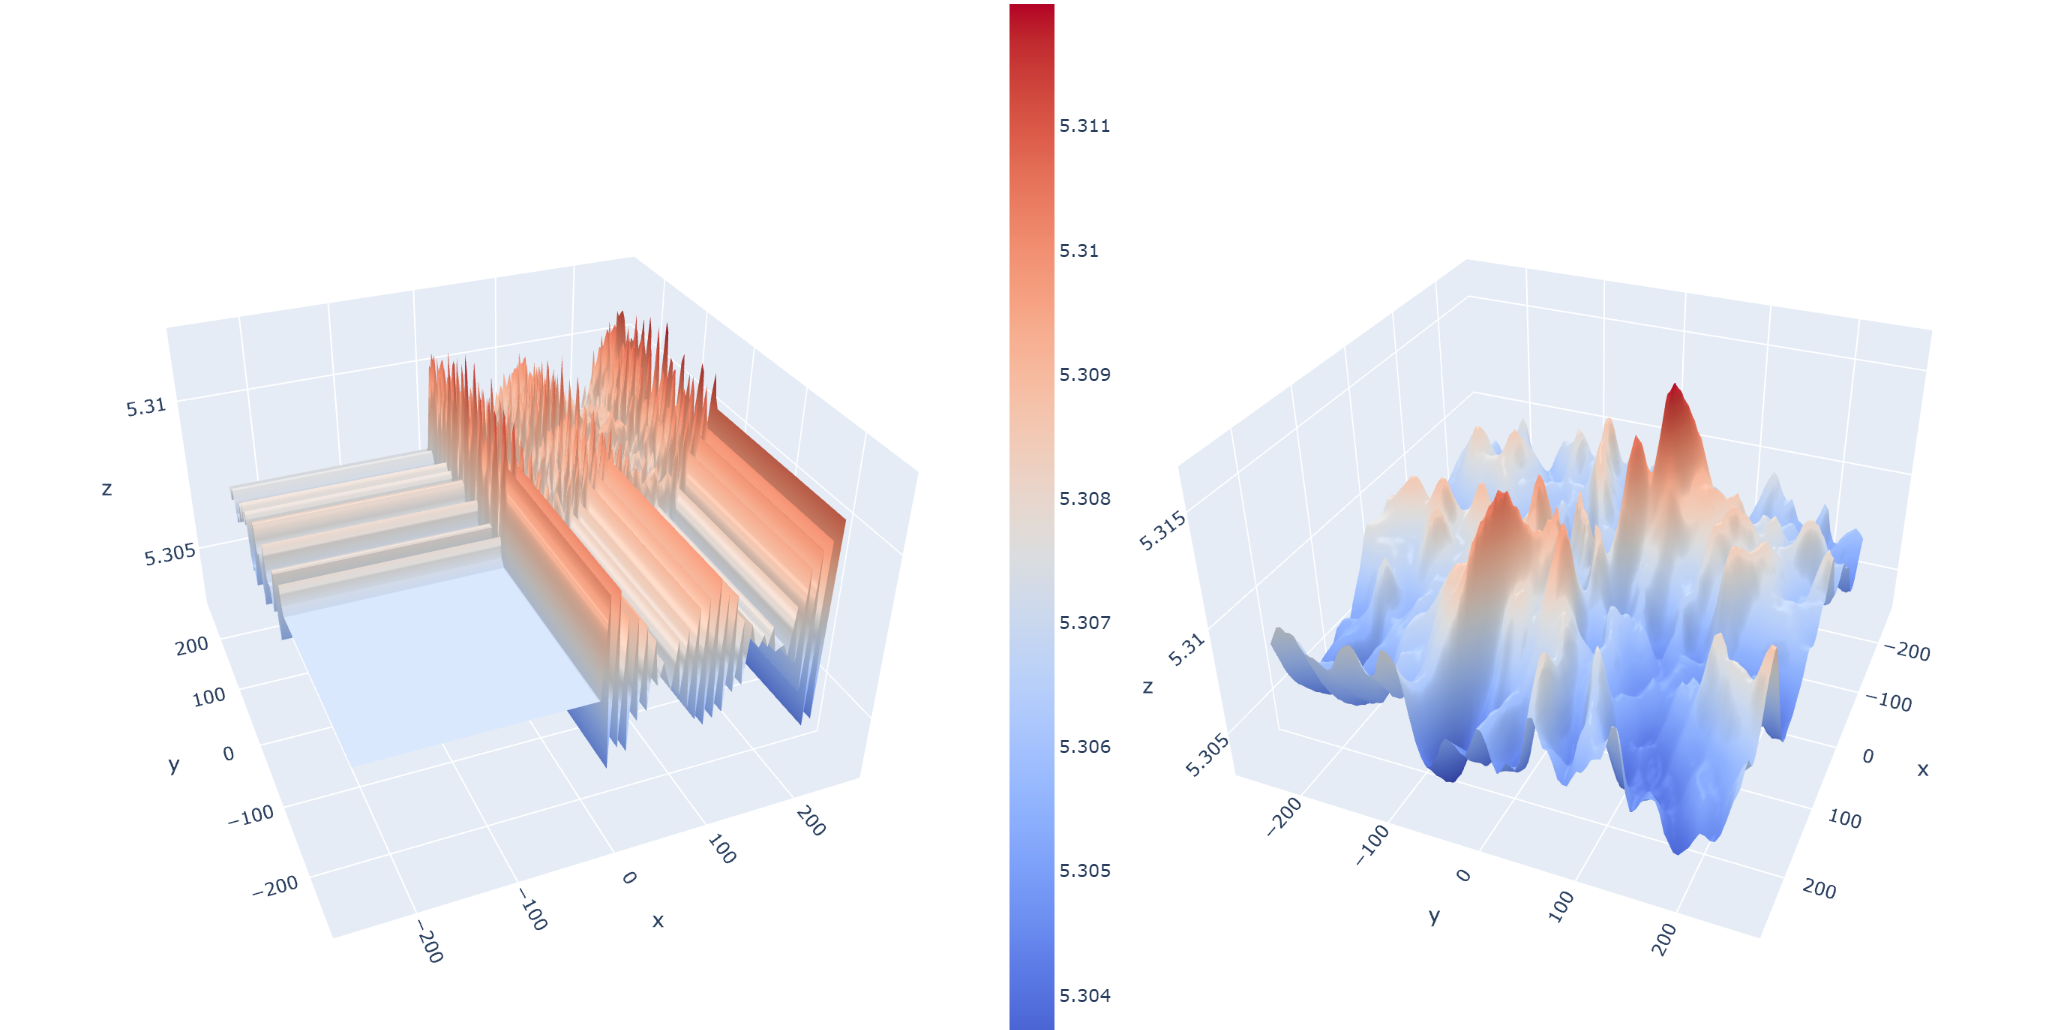
\includegraphics[width=0.8\textwidth]{figures/landscape_mmnn.png}
\caption{Landscape MMNN}
\end{figure}



Réduction paramétrique \\
$\mathcal{O}(n^2)$ vs $\mathcal{O}(n^4)$ pour FCNN

\vspace{0.5cm}

\textbf{Interprétation fréquentielle:}\\
Apprentissage de la transformée en ondelettes sur RBF\\
Performance optimale: ondelettes sparses
\end{frame}

% Slide 8: NTK pour MMNN
\begin{frame}{NTK for MMNN}

    \textbf{Architecture:} matrice milieu low-rank, train A seulement

\begin{equation}
    \bm{h}^{(\ell)}(\bm{x}) = \frac{\sigma_A}{\sqrt{n_\ell}} \sum_{j=1}^{n_\ell} \bm{A}_j^{(\ell)} \ReLU\left(\bm{w}_j^{(\ell)\top} \bm{h}^{(\ell-1)}(\bm{x}) + \beta b_j^{(\ell)}\right) + \sigma_c \bm{c}^{(\ell)}
\end{equation}



\begin{equation}
\NTK^{L}(\mathbf{x}_i, \mathbf{x}_j) = \left\langle \frac{\partial f(\mathbf{x}_i; \boldsymbol{\theta})}{\partial \boldsymbol{\theta}}, \frac{\partial f(\mathbf{x}_j; \boldsymbol{\theta})}{\partial \boldsymbol{\theta}} \right\rangle
\end{equation}

\vspace{0.5cm}

\textbf{Deux méthodes de calcul:}\\
1) TCL naïf (relation de récurrence)\\
2) Théorème d'Adler: $\textcolor{red}{\Theta_{ab}(x, x')} = \frac{\partial^2}{\partial \theta \partial \theta'} \boldsymbol{K_{ab}^{\text{NNGP}}(x, x')}$
\end{frame}

% Slide 9: Formule récursive
\begin{frame}{Formule Récursive}
\begin{equation}
\K_L^{\infty}(\mathbf{x},\mathbf{x}') = \|\mathbf{x}\| \|\mathbf{x}'\| \sum_{p=1}^{L} \varrho^{\circ (p-1)}\left( \rho_0(\mathbf{x},\mathbf{x}') \right)
\end{equation}

\begin{equation}
\varrho(\rho) = \sigma_W^2 \int \ReLU(u_1) \ReLU(u_2) d\mathcal{N}\left( [u_1,u_2] \left| 0,\left[ \begin{smallmatrix} 1 & \rho \\ \rho & 1 \end{smallmatrix} \right] \right. \right)
\end{equation}
\end{frame}
% Slide 10: Random field gaussien
\begin{frame}{Deep Gaussian Process}
\textbf{Structure du random field:}\\
Deep Gaussian = concaténation supportable

\vspace{0.5cm}

Intégrales et opérateurs de convolution\\
Analyse point fixe possible

\vspace{0.3cm}

\textbf{Formule de récursion MMNN:}
\begin{equation}
\boxed{
\Theta^{(\ell)}(x, x') = \Theta^{(\ell-1)}(x, x') \cdot \left(\sigma_A^2\dot{\Sigma}^{(\ell)}(x, x')\right) + \sigma_A^2 \Sigma^{(\ell)}(x, x') + 1
}
\end{equation}

\vspace{0.3cm}

\textbf{Validation:} prédictions théoriques vs pratique\\
Loss finale, courbures, comportement training
\end{frame}

% Slide 11: Deeper or Wider - NTK fini
\begin{frame}{Deeper or Wider? - NTK Fini}
\textbf{Réseau fini = NTK qui bouge}

$$\K_t = \K^{(0)} + \frac{1}{m}\K^{(1)}_t + \frac{1}{m^2}\K^{(2)}_t + \ldots$$

\textbf{Tenseur typique de largeur finie:}
\begin{equation}
T_{ijkl} = \frac{1}{m^2} \sum_{a=1}^m \frac{\partial^2 f_i}{\partial w_a^2} \frac{\partial^2 f_j}{\partial w_a^2} \frac{\partial f_k}{\partial w_a} \frac{\partial f_l}{\partial w_a}
\end{equation}

\vspace{0.3cm}

\textbf{Décomposition de Wick:}
\begin{align}
\mathbb{E}[X_1 X_2 X_3 X_4] &= \mathbb{E}[X_1 X_2]\mathbb{E}[X_3 X_4] \\
&+ \mathbb{E}[X_1 X_3]\mathbb{E}[X_2 X_4] \\
&+ \mathbb{E}[X_1 X_4]\mathbb{E}[X_2 X_3]
\end{align}

\vspace{0.3cm}

\textbf{Physique:} diagrammes de Feynman connectés\\
Corrélations d'ordre $2n \sim \frac{1}{m^{n/2}}$
\end{frame}
% Slide 12: Tenseurs d'ordre 3 et 4
\begin{frame}{Tenseurs d'Ordre Supérieur}
\textbf{Scaling avec la largeur:}




\textbf{Tenseur d'ordre 3:} $\textcolor{k3color}{K^{(3)}}$\\
Formulation simple obtenue

\textbf{Tenseur d'ordre 4:} complexité exponentielle\\
$\Rightarrow$ approche numérique

\vspace{0.3cm}

\textbf{Cumulants joints:}
\small{
\begin{align*}
\mathbb{E}^c[X_1, X_2, X_3] = \mathbb{E}[X_1 X_2 X_3] &- \mathbb{E}[X_1 X_2]\mathbb{E}[X_3] - \mathbb{E}[X_1 X_3]\mathbb{E}[X_2] \\
&- \mathbb{E}[X_2 X_3]\mathbb{E}[X_1] + 2\mathbb{E}[X_1]\mathbb{E}[X_2]\mathbb{E}[X_3]
\end{align*}
}

\vspace{0.2cm}

\textbf{Décomposition NTK-préactivation:}
\small{
\begin{equation*}
\mathbb{E}^c[z_{i_1}^{(\ell+1)}, z_{i_2}^{(\ell+1)}, \Delta\Theta_{i_3 i_4}^{(\ell+1)}] = \frac{1}{n_\ell} \left( D_{1234}^{(\ell+1)} \delta_{i_1 i_2}\delta_{i_3 i_4} + F_{1324}^{(\ell+1)} \delta_{i_1 i_3}\delta_{i_2 i_4} + \dots \right)
\end{equation*}
}

\vspace{0.5cm}

\textbf{Tenseur d'ordre 3:} $\textcolor{k3color}{K^{(3)}}$\\
Formulation simple obtenue

\textbf{Tenseur d'ordre 4:} complexité exponentielle\\
$\Rightarrow$ approche numérique + apport d'une méthode autodiff JAX en $m²$
\end{frame}

% Slide 13: Approche spectrale
\begin{frame}{Découverte Spectrale}
\textbf{Décomposition sur valeurs propres NTK}

\begin{equation}
\textcolor{blue!80!black}{\Theta^{(1)}_\infty(\vec{x})} = -\sum_{i=1}^N \frac{1}{\textcolor{kernelcolor}{\lambda_{i}}}(\textcolor{orange!80!black}{\mathbf{O}_{3}}(\vec{x};0)\cdot\hat{e}_{i})(\Delta f_{0}\cdot\hat{e}_{i}) + \sum_{i,j=1}^N\frac{1}{\textcolor{kernelcolor}{\lambda_{i}}(\textcolor{kernelcolor}{\lambda_{i}}+\textcolor{kernelcolor}{\lambda_{j}})}(\hat{e}_{i}^{T}\textcolor{orange!80!black}{\mathbf{O}_{4}}(\vec{x};0)\hat{e}_{j})(\Delta f_{0}\cdot \hat{e}_{i})(\Delta f_{0}\cdot \hat{e}_{j})
\end{equation}

\vspace{0.3cm}

\textbf{Scaling empirique observé:}
\begin{equation}
\mathbb{E}_{\hat{e}_i, \hat{e}_j}[(\hat{e}_{i}^{T}\textcolor{orange!80!black}{\mathbf{O}_{4}}\hat{e}_{j})(\Delta f_{0}\cdot \hat{e}_{i})(\Delta f_{0}\cdot \hat{e}_{j})] \sim \mathcal{O}\left(\frac{L^3}{N^3}\right)
\end{equation}

\vspace{0.5cm}

\textbf{Conjecture:} distribution Marchenko-Pastur\\
$\Rightarrow$ confirmée (L. Benigni et al 28/08/2025)

\textbf{Hypothèse Wigner:} espacement des valeurs propres\\
$\Rightarrow$ \textbf{validée!}
\end{frame}

% Slide 14: GOE Statistics
\begin{frame}{Random Matrix Theory}
\textbf{GOE Statistics:} répulsion des valeurs propres

%on met la figure ici
\begin{figure}
\centering

\includegraphics[width=0.8\textwidth]{figures/consecutive_spacing_ratio_dist_N64_D10_M20_L2.png}
\caption{GOE Statistics}
\end{figure}

\vspace{0.5cm}

Complexité $\mathcal{O}(m^4) \rightarrow$ forme close\\
Monte Carlo $\rightarrow$ moyenne analytique

\vspace{0.5cm}

\textbf{Structure locale + globale MP}\\
NTK calculable vs Hessienne
\end{frame}

% Slide 15: Physique statistique
\begin{frame}{Approches Physiques}
\textbf{Random Matrix Theory}\\
Combinatoire + théorème de Wick

\textbf{Field Theory}\\
Analogie systèmes en interaction

\textbf{PhysStat}\\
Système à l'équilibre, analogies verres

\vspace{0.5cm}

\textbf{Pont:} NTK, Gauss-Newton, Hessienne
\end{frame}

% Slide 16: Collaboration actuelle
\begin{frame}{Collaboration Actuelle}

\vspace{0.3cm}

\textbf{Collaborations spécifiques:}\\
• M. Guillen \& P. Misof : développements feynmaniens finite-width\\
• D. Terjek: bornes valeurs propres minimales, développement d'Hermite\\
• L. Benigni: RMT scaling avec profondeur\\
• H. Yang: transformers, S. Jun: MMNN\\
• G. Ben Arous \& S. Péché: fondements RMT\\
• Projets probabilistes futurs


\vspace{0.5cm}

\textbf{Objectif:} scaling cohérent profondeur\\
$\Rightarrow$ réponse finale loss landscape

\vspace{0.5cm}

\textbf{Suite:} statistiques locales\\
Analyse Adam \& Muon
\end{frame}

% Slide 17: Approche globale
\begin{frame}{Vision Globale}
\textbf{Communauté optimization:} NTK délaissé depuis 2022
petit regain à l'origine du RoPE beta pour SOTA llms

\begin{align}
    \bm{h}^{(\ell)}(\bm{x}) = \frac{\sigma_A}{\sqrt{n_\ell}} \sum_{j=1}^{n_\ell} \bm{A}_j^{(\ell)} \ReLU\left(\bm{w}_j^{(\ell)\top} \bm{h}^{(\ell-1)}(\bm{x}) + \beta b_j^{(\ell)}\right) + \sigma_c \bm{c}^{(\ell)} \label{eq:ntk_rope_beta}
\end{align}

\vspace{0.5cm}

\textbf{Notre approche:}\\
Coller analyses locales $\rightarrow$ globales

NTK = cuvette locale + courbure\\
\begin{align}
    f(t) &= y + e^{-\textcolor{purple}{\Theta}_{0}t}\left(1-\int_{0}^{t}dt'e^{t'\textcolor{purple}{\Theta}_{0}}\textcolor{purple}{\Theta}^{(1)}(t')e^{-t'\textcolor{purple}{\Theta}_{0}}\right)\left(f_{0}-y\right) \label{eq:evolution_solution}
    \end{align}
$t \to \infty$ en finite width = point 1, puis 2 etc .. \\
Itération $\rightarrow$ rapprocher du minimum global ?
\end{frame}

% Slide 18: Applications pratiques
\begin{frame}{Applications Pratiques}
\textbf{SciM}

Points de Chebyshev $\rightarrow$ commutation et analyse exacte\\
Bornes pratiques pour tailles et autres distributions raisonnables

\vspace{0.5cm}

\textbf{Objectif 1-2 ans:}\\ 
Librairie SciML\\
$\Rightarrow$ paramètres optimaux directs\\
Fin du trial-and-error infini depth/width
\end{frame}

% Slide 19: Leçons et documentation
\begin{frame}{Méthodologie}
\textbf{Leçon:} trouver le problème le plus trivial à résoudre, résultats rapides, 
LIRE TOUTE LA LITTERATURE malgré le flot infini

\vspace{0.5cm}

\textbf{Documentation complète:}\\
GitHub, YouTube, papiers scannés\\
$>10$ collaborations actives

\vspace{0.5cm}

\textbf{Créativité + Représentation mentale du problème}\\
\end{frame}

% Slide 20: Conclusion
\begin{frame}{Conclusion}
\begin{center}
\textbf{Contributions principales:}

\vspace{0.5cm}


Schémas numériques améliorés, résultats concrets en Sobolev training
Théorie unifiée: FCNN, MMNN, Transformers\\
Pont deep learning $\leftrightarrow$ physique mathématique = RMT
But long terme : Bornes explicites valeurs propres NTK et SGD convergence\\
\vspace{1cm}

\textbf{Résultat pratique:}\\
Guide pour choix optimal\\
\textbf{Deeper or Wider}
\end{center}
\end{frame}

\end{document}